\begin{figure}[H]
  \centering

  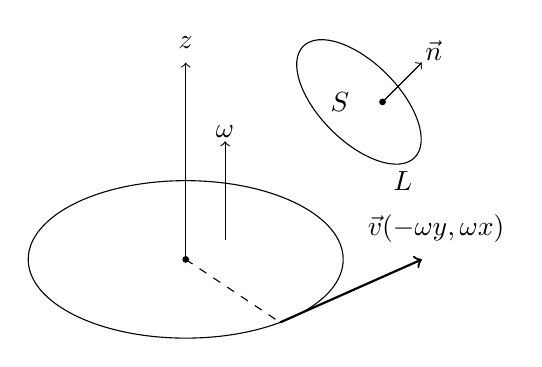
\begin{tikzpicture}
    \coordinate (P) at (1.2, -0.8);
    \draw (0, 0) ellipse (2 and 1);
    \draw[fill = black] (0, 0) circle (1pt);
    \draw[->] (0, 0) -- (0, 2.5) node[pos = 1.1] {\(z\)};
    \draw[->] (0.5, 0.25) -- (0.5, 1.5) node[pos = 1.1] {\(\omega\)};

    \draw[dashed] (0, 0) -- (P);
    \draw[thick, ->] (P) -- (3, 0)
      node[above, pos = 1.1] {\(\vec{v} (-\omega y, \omega x)\)};

    \draw[rotate around = { 135 : (2.2, 2) }]
      (2.2, 2) ellipse (1 and 0.5);
    \draw node[left] at (2.2, 2) {\(S\)};
    \draw node[left] at (3, 1) {\(L\)};

    \draw[fill = black] (2.5, 2) circle (1pt);
    \draw[->] (2.5, 2) -- (3, 2.5)
      node[pos = 1.3] {\(\vec{n}\)};
  \end{tikzpicture}
\end{figure}
